% 第 12 章 Creating Charts
\bichapter{创建图表}{Creating Charts}
\label{chap:gui-chart}

IC Compiler II 工具包含一套完整的绘图生成功能，可根据设计、版图及其他数据生成交互式绘图（plot）。更多信息见下列主题：
\begin{itemize}
  \item 创建模型
  \item 创建绘图
\end{itemize}

\section{创建模型}
\subsection*{Creating a Model}

要创建图表（chart），先从逗号分隔值（comma-separated values，CSV）文件导入图表数据，以创建模型（model）。使用 \cmd{gui\_create\_charts\_model} 命令读取 CSV，并把信息保存为 Tcl 变量。

下例写出一个简单的 CSV 文件，其中包含设计里每个宏单元（macro）的实例名、管脚数和面积。\cmd{gui\_create\_charts\_model} 命令装入该 CSV 文件并创建图表模型。

\begin{lstlisting}
set macros [get_cells -hier -filter "design_type==macro"]
set csv_file /tmp/count_area.csv
echo "macro_inst,count,area" > $csv_file
foreach_in_collection c $macros {
  echo [get_object_name $c],[get_attribute $c number_of_pins],[get_attribute $c area] >> $csv_file
}
set model [gui_create_charts_model -csv $csv_file -first_line_header ]
\end{lstlisting}

\begin{noteBox}
\cmd{gui\_create\_charts\_model} 命令会自动推导每一列数据的数据类型（data type）。
\end{noteBox}

也可以用 GUI 导入 CSV 文件。在 View Settings 面板中单击 Charts 选项卡，再单击 Models 选项卡。单击 Create 按钮，打开 Load Model 对话框。输入文件名，并选择用于指定表头的选项。工具会显示数据预览，见图~\ref{fig:gui-143}。单击 OK 创建模型。

\begin{figure}[htbp]
\centering
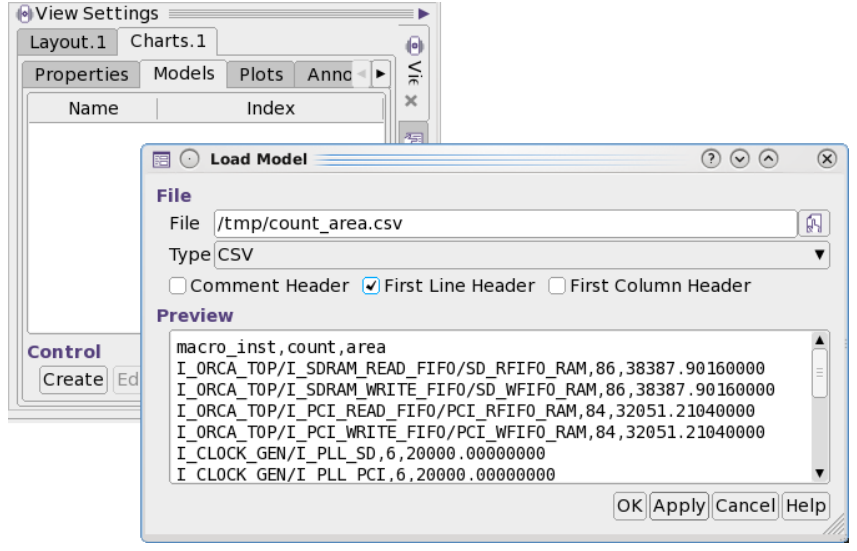
\includegraphics[width=0.92\textwidth]{gui-fig-143.png}
\caption{Load Model 对话框}
\label{fig:gui-143}
\end{figure}

除 CSV 之外，还可以直接从集合（collection）或 Tcl 数组（Tcl array）创建模型。例如：

\begin{lstlisting}
set selection [get_nets]
set model1 [gui_create_charts_model -clct $selection -columns {name dr_x_length dr_y_length}]

set data [list \
[list State {Under 5 Years} {5 to 13 Years} {14 to 17 Years} {18 to 24 Years} {25 to 44 Years} {45 to 64 Years} {65 Years and Over}] \
[list CA 2704659 4499890 2159981 3853788 10604510 8819342 4114496] \
[list TX 2027307 3277946 1420518 2454721 7017731 5656528 2472223] \
[list NY 1208495 2141490 1058031 1999120 5355235 5120254 2607672] \
[list FL 1140516 1938695 925060 1607297 4782119 4746856 3187797] \
[list IL 894368 1558919 725973 1311479 3596343 3239173 1575308] \
[list PA 737462 1345341 679201 1203944 3157759 3414001 1910571] \
]

set model2 [gui_create_charts_model -tcl $data -first_line_header]
\end{lstlisting}

\subsection{检查模型}
\subsubsection*{Checking the Model}

创建模型之后，在 GUI 中检查该模型：单击 View Settings 面板中的 Charts 选项卡。单击 Models 选项卡，显示用 \cmd{gui\_create\_charts\_model} 命令创建的模型列表。

要查看某个模型的详细信息，包括列名、数据类型和其他属性，在表中单击该模型，再单击 Edit 按钮，以显示数据表。单击每一列，可显示该数据列的列名、数据类型和其他属性。要更改该列的属性，在 Column Data 区域中选择一项，再单击 Apply。

\begin{figure}[htbp]
\centering
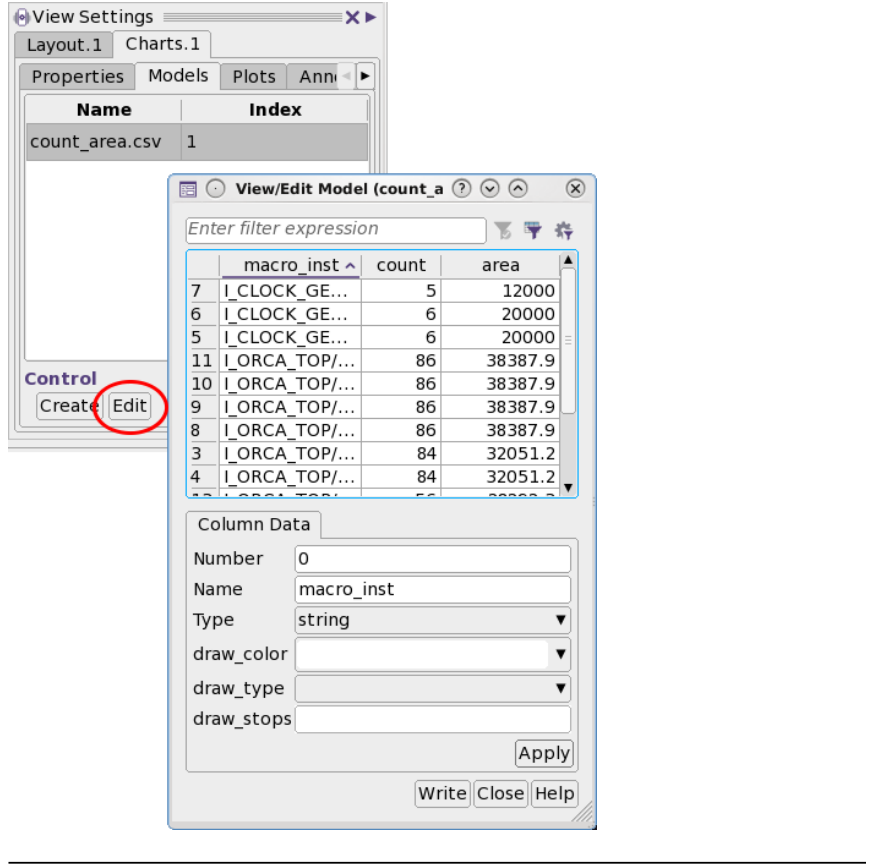
\includegraphics[width=0.92\textwidth]{gui-fig-144.png}
\caption{View/Edit Model 对话框}
\label{fig:gui-144}
\end{figure}

\subsection{向模型添加或删除数据}
\subsubsection*{Adding or Deleting Data From the Model}

导入 CSV 文件之后，可以用 \cmd{gui\_change\_charts\_model} 命令修改数据：添加列、删除列，以及执行其他操作。下例添加名为 \cmd{double\_count} 的新列，其值是 \cmd{column(1)} 中数据的两倍。

\begin{lstlisting}
gui_change_charts_model -model $model -add \
   -expr {column(1) + column(1)} -header double_count
\end{lstlisting}

\section{创建绘图}
\subsection*{Creating a Plot}

导入 CSV 文件并创建模型之后，可以创建绘图来查看数据。使用 \cmd{gui\_create\_charts\_plot} 命令创建条形图（bar chart）、分布图（distribution plot）、XY 图表（XY chart）等。

下例写出一个 CSV 文件，其中包含设计里四个宏单元的管脚数与面积。\cmd{gui\_create\_charts\_plot} 命令根据 CSV 文件的内容创建初始绘图。接着，从上下文菜单（context menu）中选择 Horizontal，把绘图转换成水平条形图。从上下文菜单中选择 Show Table，以显示数据表。

\begin{lstlisting}
# Create the Charts window
set view [gui_create_window -type Charts]

# Specify the macros and output CSV file
set macros [get_cells { cmem0/idata0_2/x0_t0 cmem0/dtags1_1/x0_t0
                        rf0/x0/t_bl cmem0/itags0_3/x0_t0 }]
set csv_file count_area.csv

# Write out the CSV file
echo "macro_inst,count,area" > $csv_file
foreach_in_collection c $macros {
  echo [get_object_name $c],\
[get_attribute $c number_of_pins],\
[get_attribute $c area] >> $csv_file
}

# Create the model
set model [gui_create_charts_model -csv $csv_file -first_line_header]

# Create the bar chart from the model
set plot [gui_create_charts_plot -view $view -type barchart \
   -model $model -columns {{name 0} {value {1}}}]
\end{lstlisting}

\begin{figure}[htbp]
\centering
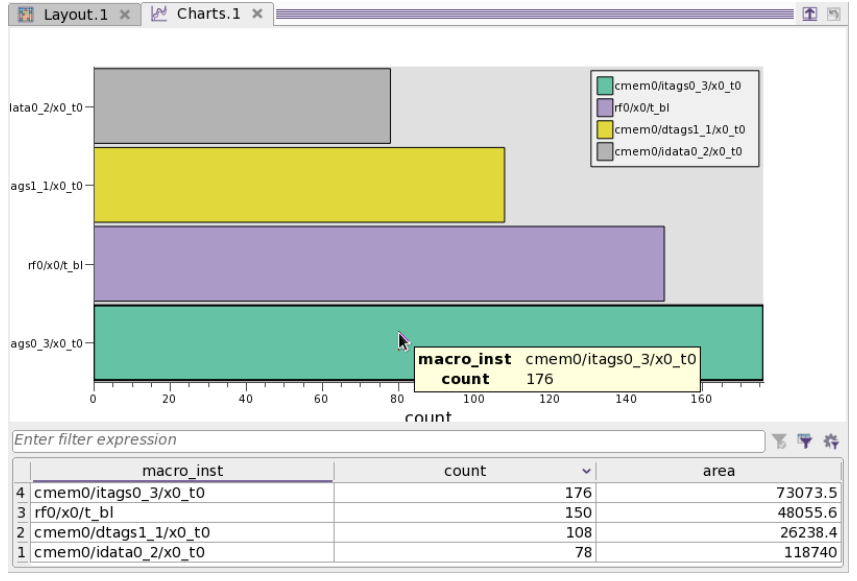
\includegraphics[width=0.92\textwidth]{gui-fig-145.png}
\caption{条形图}
\label{fig:gui-145}
\end{figure}

创建图表之后，单击列标题可以对数据排序。要过滤表中的数据，在过滤表达式框中输入过滤表达式。例如，只显示 count 大于 100 的宏单元时，在过滤表达式框中输入“count > 100”，见图~\ref{fig:gui-146}。

\begin{figure}[htbp]
\centering
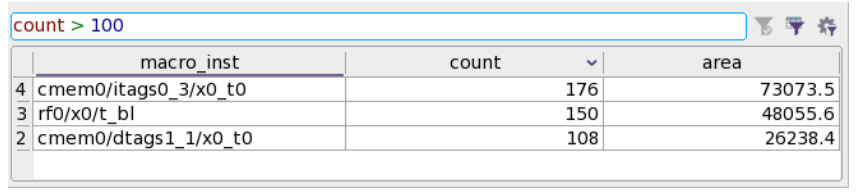
\includegraphics[width=0.92\textwidth]{gui-fig-146.png}
\caption{过滤绘图数据}
\label{fig:gui-146}
\end{figure}

\subsection{定制绘图}
\subsubsection*{Customizing a Plot}

可以修改绘图，以便：
\begin{itemize}
  \item 用 \textbf{View Settings > Properties} 或 \cmd{gui\_set\_charts\_property} 命令定制外观
  \item 用 \textbf{View Settings > Annotations} 或 \cmd{gui\_create\_charts\_*\_annotation} 命令添加标注
  \item 用 \textbf{View Settings > Plots}，或 \cmd{gui\_place\_charts\_plots} 与 \cmd{gui\_group\_charts\_plots} 命令，在视图中排布多个绘图
  \item 用 \cmd{gui\_connect\_charts\_signal} 命令，在用户交互时运行自定义 Tcl 过程
\end{itemize}
